During the first two runs of the CERN Large Hadron Collider (LHC)~\cite{Evans:2008zzb}, experimental collaborations, such as the ATLAS~\cite{ATLAS:2008xda} and CMS~\cite{CMS:2008xjf} Collaborations, have analyzed trillions of high energy proton-proton collisions and produced an extensive suite of physics results. Among these are the discovery of the Higgs boson~\cite{ATLAS:2012yve,CMS:2012qbp} in the standard model (SM),  and world-leading constraints on various beyond the SM (BSM) physics scenarios, such as supersymmetry~\cite{ATLAS:2021hza, ATLAS:2021twp, ATLAS:2021kxv, CMS:2020fia, CMS:2021edw, CMS:2022vpy} and exotic heavy-particle or dark matter candidate productions~\cite{ATLAS:2022ozf, ATLAS:2021wob, CMS:2022usq, CMS:2022qej}. In order to pursue further SM measurements and BSM searches, the amount of data the LHC delivers and the associated data processing rates of the experiments are expected to increase dramatically in upcoming physics runs~\cite{Bruning:2015dfu}.

The high data-taking rates of ATLAS and CMS, which are currently in the range of 0.1--1\unit{PB/s} and planned to increase to $\mathcal{O}(10)\unit{PB/s}$, present a significant computational challenge for physicists to process the data~\cite{Zabi:2020gjd,2137107}. 
%Because it is neither feasible nor desirable to store such large volumes of data, both experiments employ two-level trigger systems to reduce the final rate to about 10\unit{GB/s}~\cite{ATLAS:2020esi, CMS:2016ngn}, often referred to as ``online''. After raw data is stored, it is processed to extract high-level information that is useful for analysis, referred to as ``offline''. 
A two-level trigger system is employed to run fast algorithms and reduce the data rate to about 10\unit{GB/s}~\cite{ATLAS:2020esi, CMS:2016ngn}; while this is a significantly smaller rate, it is still very challenging for subsequent processing steps. As shown in Fig.~\ref{fig:CPU_needs}, even with aggressive computing research and development and favorable budget increases, the projected computing needs for CMS will be only narrowly satisfied.

\begin{figure}[htp]
    \centering
    %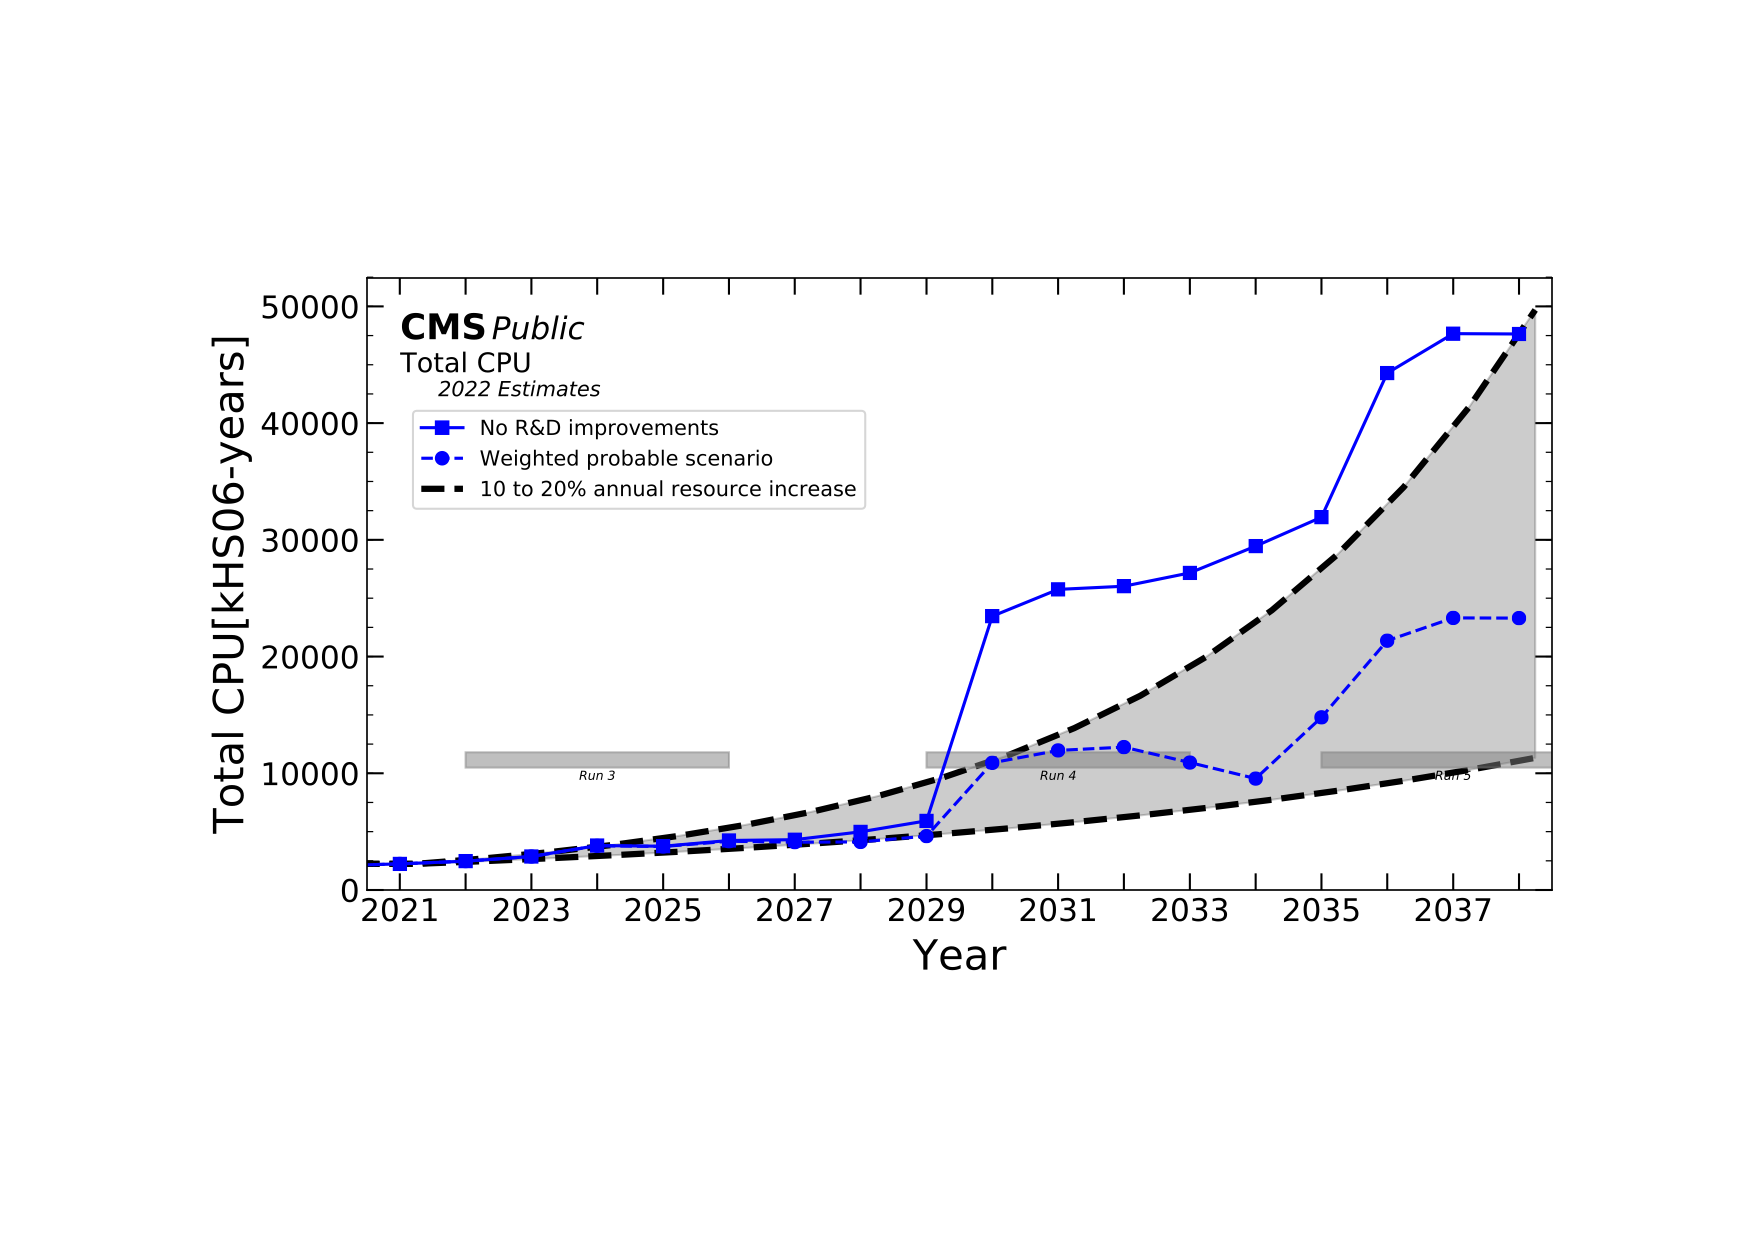
\includegraphics[height=7cm,trim={1cm 4cm 0 4cm},clip]{plots/cpu_cms2022.pdf}
    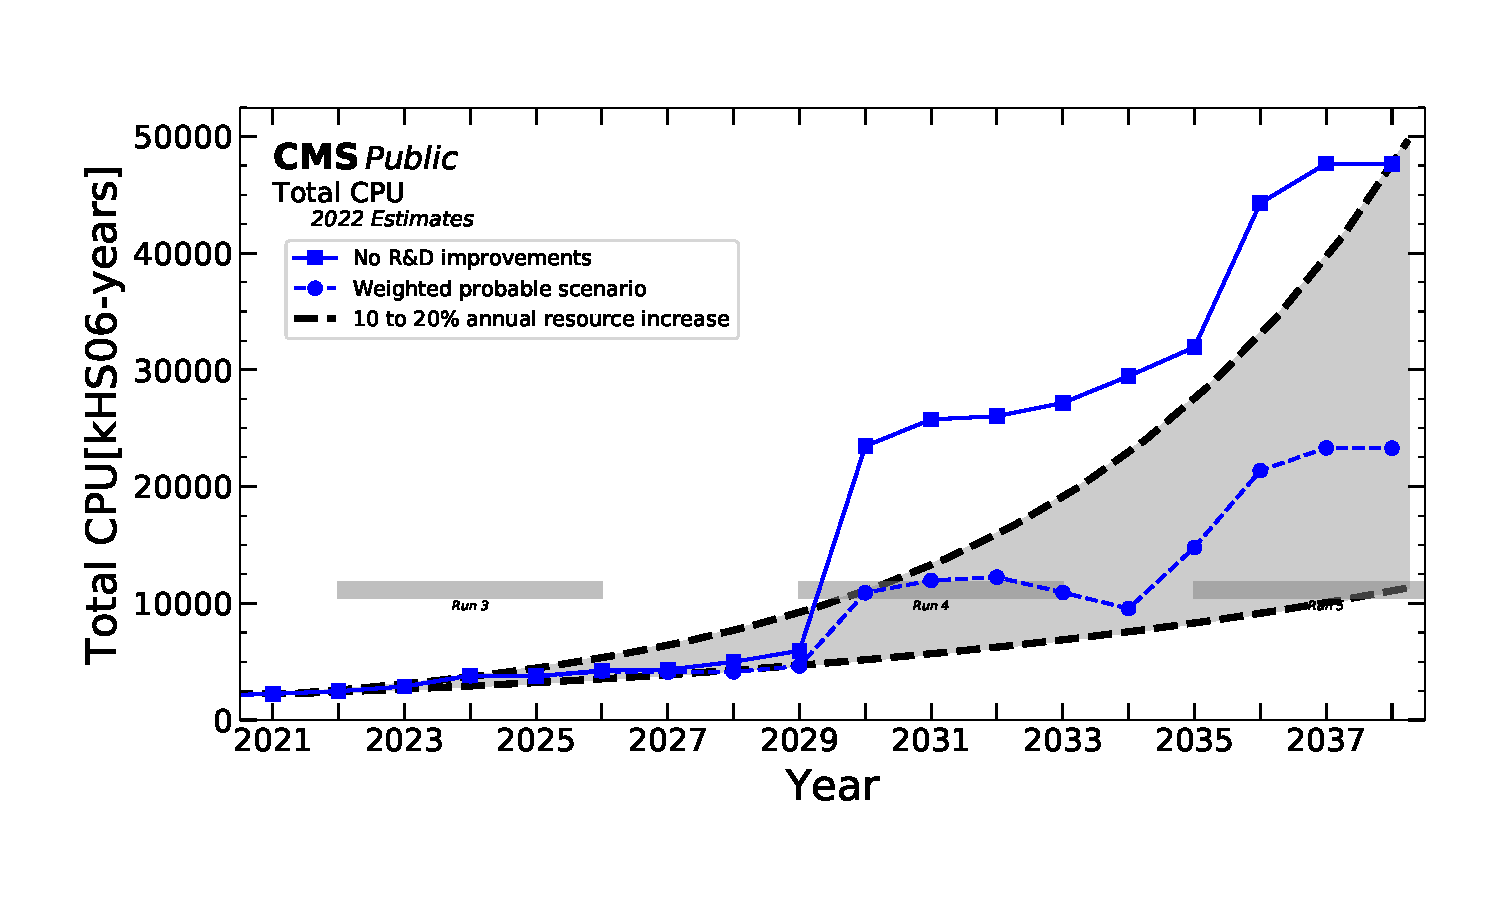
\includegraphics[height=7cm,trim={0 1cm 0 1cm},clip]{plots/cpu_cms2022_vectorized.pdf}
    %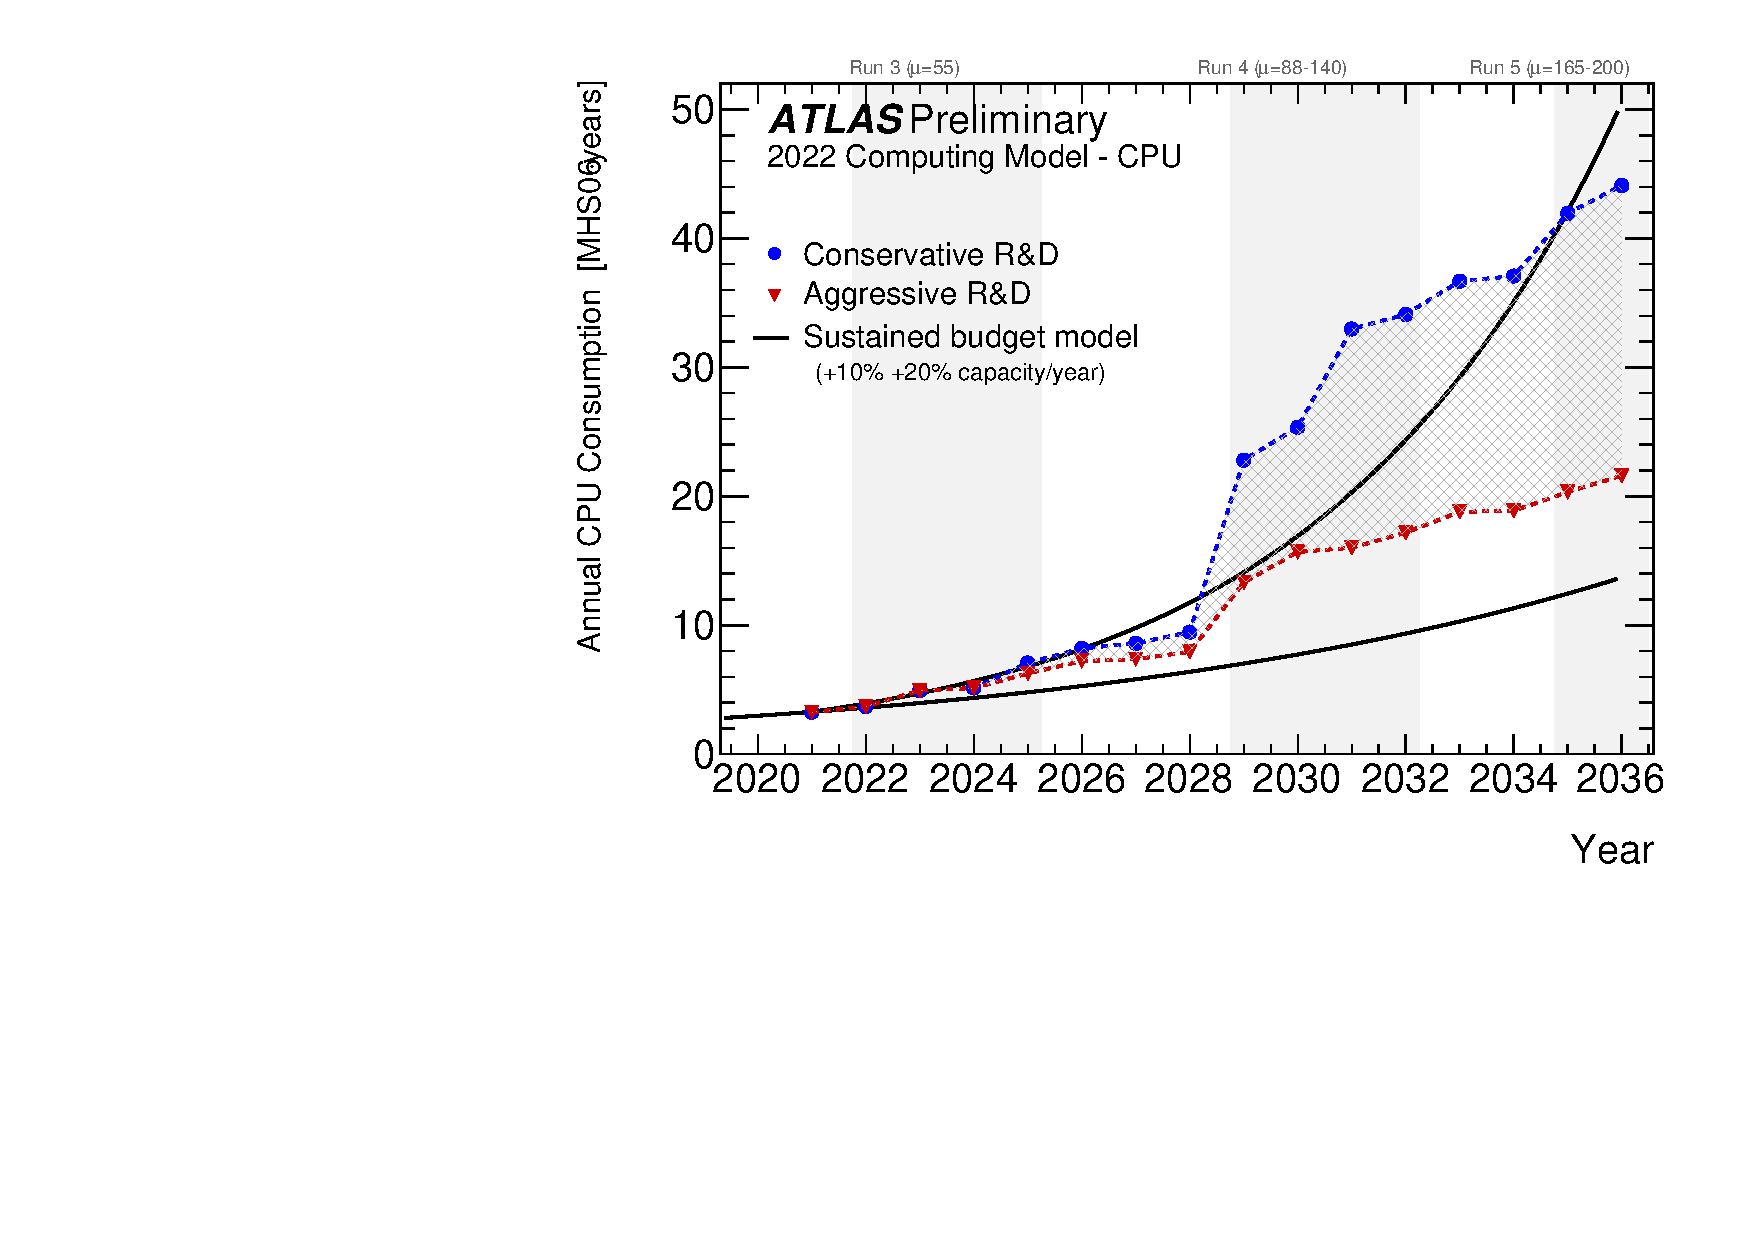
\includegraphics[width=0.75\textwidth]{plots/cpu_atlas2022.pdf}
    \caption{CPU time requirement projections for CMS offline processing and analysis needs~\cite{CMS_computing_plot, CMS:2815292}. Plot shows projected resource availability based on 10\% and 20\% annual budget increases. Lines are included for projections based on current performance and performance with expected research and development improvements. An analogous plot from ATLAS can also be found in Ref.~\cite{ATLAS_computing_plot}. }
    \label{fig:CPU_needs}
\end{figure}

\begin{sloppypar}While the expected performance increase of CPUs is limited, data processing can also be carried with a variety of modern architectures, such as graphics processing units (GPUs), field-programmable gate arrays (FPGAs), and application-specific integrated circuits (ASICs), which can collectively be referred to as ``coprocessors.'' These architectures are becoming increasingly popular because of their large numbers of processing units and inherent parallelization designs, especially suited for machine learning (ML) algorithm computations. Previous studies have shown that running ML algorithm inference on coprocessors can dramatically reduce the computation latency and increase the throughputs for high energy physics (HEP) data processing~\cite{Duarte:2019fta, Krupa:2020bwg, Wang:2020fjr}. In addition, it is also possible to design domain algorithms that are specifically optimized for coprocessor acceleration, such as ``Patatrack,'' which is designed to run in a heterogeneous architecture in the CMS high-level trigger (HLT) system, reducing the per-event latency of the trigger~\cite{Bocci:2020pmi}.\end{sloppypar}

Within HEP, deep learning (DL) algorithms are already widely used for regression and classification tasks, and their popularity is growing rapidly~\cite{Guest:2018yhq, Albertsson:2018maf, Bourilkov:2019yoi, Larkoski:2017jix}. These algorithms can be easily accelerated on heterogeneous architectures and are taking up increasing fractions of the overall processing loads. Therefore, developing a framework to enable and optimize the deployment and portability for coprocessors is of considerable interest to HEP experiments.

The most straightforward framework for deployment is to simply equip every CPU machine with coprocessors, referred to as ``directly-connected." In this scenario, every CPU thread within the machine can communicate with the coprocessor. However, since communications are limited to the CPUs and coprocessors within the same machine, it is hard to explore additional or different types of coprocessor resources. Besides, since the CPU-coprocessor ratio needs to be predetermined and fixed after deployment, the coprocessor resources are unlikely to be optimally utilized, leading to either wasted cost when under-saturating, or performance drops when over-saturating.

An alternative framework is ``inference as a service'' (IaaS), where coprocessor resources are factorized out of CPU machines. As represented in Fig.~\ref{fig:illustration}, in this scheme \emph{CPU-based clients} can send the computing request with necessary information to \emph{coprocessor-based servers} via network calls; servers running on coprocessor resources can perform computing tasks upon request. This removes the restriction of a coprocessor only being used by the CPUs directly connected to it, allowing it to accept processing requests from any CPUs (local or remote) as long as network communications are guaranteed. Certain types of coprocessors can be allocated for specific tasks, and the CPU-coprocessor ratio is flexible and dynamic. Resource utilization can therefore be optimized based on specific tasks, as the number of client-side jobs using a single server can be scaled up or down depending on the computational demands of a given task. Furthermore, at the software level, since the supports for coprocessors and CPU workflows are separated, it becomes much easier to support different types of coprocessors. This ensures algorithm portability with minimal development or maintenance burden.

\begin{figure}[htp]
    \centering
    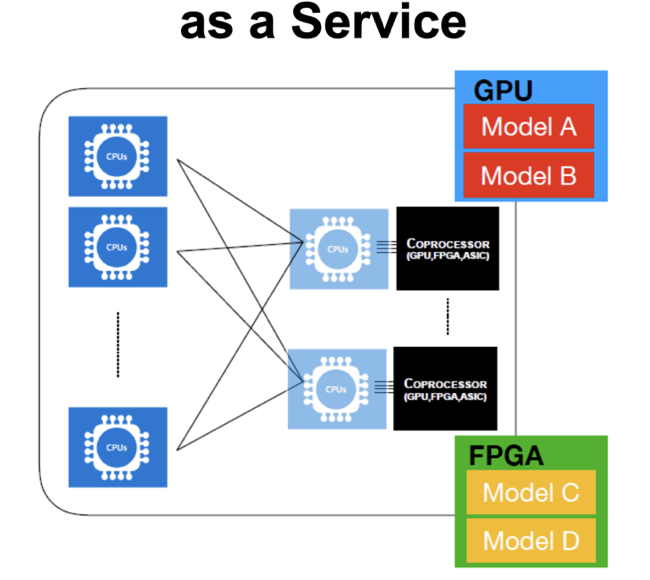
\includegraphics[width=0.50\textwidth]{plots/illustration.png}
    \caption{An illustration of an example inference as-a-service setup with multiple coprocessor servers. (\textcolor{red}{This plot will be updated to have a better quality.})}
    \label{fig:illustration}
\end{figure}

%Mention SONIC?

In this paper, we take the CMS Mini-AOD data processing~\cite{Petrucciani:2015gjw} as an example, and explore the performance benefits of employing the IaaS framework in it. In the current CMS Mini-AOD processing workflow, about 10\% of the computing time is consumed by ML algorithm inferences, which can be easily accelerated on GPUs. We firstly summarize studies of the optimization and acceleration of the inference of each individual ML algorithm on GPUs. Then we show that the IaaS scheme, which is implemented in the CMS software framework \CMSSW~\cite{CMS:2006myw} via the Services for Optimized Network Inference on Coprocessors (SONIC) approach~\cite{Krupa:2020bwg}, not only decreases processing latency but can also be deployed in large-scale productions to optimize GPU utilization. Finally we show that the SONIC approach can be easily ported to different types of coprocessors, and run as well on local CPUs without performance decrease.

The paper is organized as follows. Section~\ref{sec:cmscomputing} briefly goes through prior work to optimize ML algorithms on GPUs with IaaS. Section~\ref{sec:sonic} provide a more detailed introduction to SONIC. Section~\ref{sec:algo} discusses the Mini-AOD workflow used as a demonstration for SONIC and the algorithms that are to be accelerated on GPUs.
Algorithm optimization and performance results from the Mini-AOD tests are then shown in Section~\ref{sec:performances}. Portability to different types of processors, including local CPUs and Graphcore Intelligence Processing Units (IPUs)~\cite{Graphcore, IPU_Perf} coprocessors is presented in Section~\ref{sec:IPUs}. Finally, Section~\ref{sec:summary} summarize the studies and discusses future plans.